% =====================================================================
%  A deformability threshold for stiffness-based sorting in DLD devices
%  Target journal: Microfluidics and Nanofluidics (Springer)
%
%  Build:
%      pdflatex main && bibtex main && pdflatex main && pdflatex main
%  or:
%      latexmk -pdf main.tex
%
%  For the actual M&N submission, swap the documentclass for the
%  Springer Nature template (sn-jnl.cls) — see the commented block
%  below. The article class used here renders identically for review.
% =====================================================================

% ----------- Springer Nature M&N submission template ---------------
% \documentclass[sn-mathphys-num]{sn-jnl}
% (download sn-jnl.cls + sn-mathphys.bst from
%  https://www.springernature.com/gp/authors/campaigns/latex-author-support)
% --------------------------------------------------------------------

\documentclass[11pt,a4paper]{article}

\usepackage[T1]{fontenc}
\usepackage[utf8]{inputenc}
% Note: lmodern is recommended if available
%   (better text rendering at all sizes); falls back to Computer Modern.
% microtype is only loaded if lmodern is — microtype's auto-expansion
% requires scalable Type-1 fonts.
\IfFileExists{lmodern.sty}{%
  \usepackage{lmodern}%
  \IfFileExists{microtype.sty}{\usepackage{microtype}}{}%
}{}
\usepackage[english]{babel}
\usepackage[a4paper,margin=2.4cm]{geometry}
\usepackage{amsmath, amssymb, amsfonts}
\usepackage{graphicx}
\usepackage{booktabs}
\usepackage{xcolor}
\usepackage[colorlinks=true,
            linkcolor=blue!50!black,
            citecolor=blue!50!black,
            urlcolor=blue!50!black]{hyperref}
\usepackage{caption}
\captionsetup{font=small,labelfont=bf,labelsep=period}
\usepackage{authblk}
\IfFileExists{lineno.sty}{\usepackage{lineno}}{}
\IfFileExists{setspace.sty}{\usepackage{setspace}}{}

\graphicspath{{figures/}}

% --------- Citation style (numeric, M&N default) -----------
\usepackage[numbers,sort&compress]{natbib}
% plainnat ships with natbib and is universally available.
% For the M&N submission, swap to the Springer basic style:
%   \bibliographystyle{spbasic}
% (Springer provides spbasic.bst with the sn-jnl template — drop it
%  in the same directory as main.tex and rebuild.)
\bibliographystyle{plainnat}

% --------- Authorship -----------
\title{\textbf{A deformability threshold for stiffness-based sorting
       in deterministic-lateral-displacement microfluidic devices:
       a 2D lattice-Boltzmann immersed-boundary parameter sweep}}

\author[1]{Ram Chand\thanks{Corresponding author:
   \texttt{ram.chand@bnbwu.edu.pk}}}
\affil[1]{Department of Natural Sciences,
   The Begum Nusrat Bhutto Women University,
   Sukkur, Sindh, Pakistan}

\date{\today}

% --------- Line numbers for review (comment out before submission) ---
\makeatletter
\@ifpackageloaded{lineno}{\linenumbers}{}
\@ifpackageloaded{setspace}{\onehalfspacing}{}
\makeatother

% =====================================================================
\begin{document}
% =====================================================================

\maketitle

% ---------------------------------------------------------------------
\begin{abstract}
\noindent Deterministic lateral displacement (DLD) is the workhorse
passive-sorting technology in microfluidic cell-separation chips, but
the classical Huang--Holm critical-bin theory was derived for rigid
spheres. Recent experimental and computational work has shown that
deformable particles can be sorted by stiffness at identical particle
size, opening the door to label-free, mechanophenotyping-based
separation of red blood cells, circulating tumour cells and synthetic
vesicle carriers. The quantitative conditions under which stiffness
alone is sufficient to drive sorting, however, remain unclear. Here
we use an open-source 2D lattice-Boltzmann immersed-boundary engine
with Skalak-membrane capsules (\textsc{SoftFlow}) to perform a
systematic upper-triangle parameter sweep over 15
$(G_s^{\text{soft}}, G_s^{\text{stiff}})$ pairs spanning a
$27\times$ stiffness contrast, with all other membrane parameters
matched so the diagonal $G_s^{\text{soft}} = G_s^{\text{stiff}}$ is a
strict no-contrast control. The diagonal-subtracted DLD
displacement-angle separation,
$\Delta\theta_{\text{corr}}$, isolates the pure deformability
contribution from the finite-$N$ statistical baseline. We identify a
clear \emph{deformability threshold}: stiffness-based sorting emerges
only when the soft-species Capillary number exceeds
$\mathrm{Ca}_{\text{soft}} \approx 0.2$, below which both species
traverse the array as effectively rigid spheres and the geometric DLD
selection rule applies to both regardless of contrast. Above the
threshold, $|\Delta\theta_{\text{corr}}|$ grows with the stiffness
ratio and saturates near a ratio of $\sim 13$. This practical design
rule --- operate at $\mathrm{Ca}_{\text{soft}} > 0.2$ for
deformability sorting --- directly informs chip parameter selection
(pillar gap, throughput, target cell type). We release the full
LBM-IBM engine, the per-cell \verb|run_manifest.json| provenance
records and the analysis pipeline as a reusable open-source resource
for community parameter sweeps.

\vspace{1em}
\noindent\textbf{Keywords:}
deterministic lateral displacement~\textperiodcentered~
capillary number~\textperiodcentered~
capsule deformability~\textperiodcentered~
lattice Boltzmann method~\textperiodcentered~
immersed boundary method~\textperiodcentered~
cell sorting~\textperiodcentered~
microfluidics~\textperiodcentered~
open-source software
\end{abstract}

% ---------------------------------------------------------------------
\section{Introduction}
\label{sec:intro}

Deterministic lateral displacement
(DLD)~\citep{huang2004continuous,davis2006deterministic} sorts
suspended particles by size using a parallelogram lattice of
micropillars whose row-to-row lateral shift~$\delta$ defines a
\emph{critical bin} diameter $D_c$. Particles larger than $D_c$ are
``bumped'' laterally one row per column ---  the so-called
displacement mode --- while smaller particles execute a zigzag
trajectory and recover their initial streamline after a full lattice
period. The original derivation by Davis and
co-workers~\citep{davis2006deterministic,inglis2006critical} assumed
rigid spherical particles, and Holm and co-workers later refined the
critical-size formula to $D_c \approx 1.4\,G\,\sqrt{\delta/\Delta x}$
for hard spheres in symmetric arrays~\citep{holm2011separation},
where $G$ is the lateral pillar gap and $\Delta x$ the column
spacing. This rigid-sphere theory has been verified
experimentally~\citep{mcgrath2014deterministic} and is now the
working basis of clinical DLD chips for circulating-tumour-cell
enrichment and red-blood-cell fractionation.

A growing body of work shows that the rigid-sphere assumption breaks
down for biological cells, whose deformability fundamentally alters
their interaction with the obstacle
array~\citep{quek2011separation,beech2012sorting,zhang2015behavior}.
Henon et al.~\citep{henon2017deterministic} demonstrated
experimentally that softer red blood cells migrate at a smaller
effective displacement angle than stiffer ones \emph{at identical
size}, opening DLD to mechanophenotyping. On the computational side,
Vahidkhah and Bagchi~\citep{vahidkhah2015microparticle} used 3D
boundary integral simulations to show that capsule shape and
deformability shift the critical bin by 10--40\,\% depending on
Capillary number, and D'Avino and
Maffettone~\citep{davino2015particle} reviewed the broader class of
softness-driven migration in confined microchannel flows.

What remains poorly mapped is the \emph{threshold} behaviour: at
which value of the soft-species Capillary number,
$\mathrm{Ca}_{\text{soft}}$, does deformability begin to contribute
appreciably to sorting? Below the threshold, both soft and stiff
particles should behave as effectively rigid and any stiffness
contrast should be irrelevant. Above it, a chip operating in
deformability-sorting mode should display a monotonically increasing
displacement-angle separation with stiffness ratio. The threshold
itself is the key engineering design rule for any DLD device
targeting mechanophenotyping --- it sets the minimum required flow
speed (and hence chip throughput) for a given target cell type, or
conversely the maximum allowed stiffness for which sorting is
feasible at a given throughput.

This study reports a systematic 2D lattice-Boltzmann
immersed-boundary parameter sweep over a five-by-five grid of soft
and stiff shear-elastic moduli, with all other capsule mechanical
parameters held identical so that the diagonal of the grid is a
strict no-contrast control. We introduce a diagonal-subtracted
displacement-angle separation,
$\Delta\theta_{\text{corr}}$, that isolates the pure deformability
contribution from the finite-$N$ noise inherent in any
particle-resolved suspension simulation, and we identify a
deformability threshold at $\mathrm{Ca}_{\text{soft}} \approx 0.2$
above which sorting emerges. We release the full simulation engine,
the analysis pipeline, and per-cell provenance records
(\verb|run_manifest.json| with git commit, compiler flags, full
resolved configuration and RNG seed) as an open-source resource so
that the parameter sweep can be extended by the community without
re-implementation.

The remainder of this paper is organised as follows.
Section~\ref{sec:methods} describes the LBM-IBM engine, the capsule
membrane model, the DLD geometry, and the sweep design including the
randomised-order singleton seeding protocol we developed to remove
two-pass RSA bias. Section~\ref{sec:results} reports the diagonal
noise-floor characterisation, the corrected angular separation, and
the Capillary-number collapse that identifies the threshold.
Section~\ref{sec:discussion} compares the threshold to published 3D
data and discusses limitations. Section~\ref{sec:conclusion}
summarises the design rule and outlines future work.

% ---------------------------------------------------------------------
\section{Methods}
\label{sec:methods}

\subsection{Fluid solver: D2Q9 lattice Boltzmann}
\label{sec:methods-lbm}

The fluid is solved using the D2Q9 lattice Boltzmann method
\citep{kruger2017lattice}. We use the regularised BGK collision
operator of Latt and Chopard~\citep{latt2006lattice}, which damps
non-equilibrium ghost modes and substantially improves stability at
the moderate relaxation time
($\tau = 0.70$, corresponding to lattice kinematic viscosity
$\nu = (\tau - 1/2)/3 = 0.067$ in lattice units) used throughout the
sweep. Periodic boundary conditions are imposed in $x$ and no-slip
walls (halfway bounce-back) in $y$. Solid pillar obstacles employ
the interpolated bounce-back scheme of Bouzidi, Firdaouss and
Lallemand~\citep{bouzidi2001momentum} for second-order accurate
treatment of the curved surfaces. The flow is driven by a constant
body force $F_x = 3 \times 10^{-5}$ lattice units (LU), giving a
centre-line Poiseuille velocity of
$U_c \approx F_x H^2 / (8\nu) \approx 0.035$ LU in the absence of
pillars and capsules. The lattice Mach number remains $\mathrm{Ma}
\lesssim 0.06$ throughout, well within the incompressibility regime.

\subsection{Fluid--particle coupling: immersed boundary method}
\label{sec:methods-ibm}

The capsule membranes are coupled to the fluid via the immersed
boundary method~\citep{peskin2002immersed} with
multi-direct-forcing iterations~\citep{luo2007numerical}: the
spreading-and-interpolation cycle is repeated twice per time step,
which reduces the residual no-slip violation at the membrane by an
order of magnitude relative to single-pass IBM. The regularised
delta function is the four-point Peskin
kernel~\citep{peskin2002immersed}. A force-cap of 0.04~LU per node
per step is applied to guard against pathological excursions; in
practice this limit is never reached at the parameters used here.

\subsection{Capsule membrane model}
\label{sec:methods-membrane}

Each capsule is discretised as a closed polygon of
$N_{\text{node}} = 18$ membrane nodes connected by Skalak-style
springs~\citep{skalak1973strain}, with bending resistance
implemented as a Helfrich-style angular potential between adjacent
node triples. The Skalak strain-energy density is
\begin{equation}
  W_{\text{Skalak}} = \tfrac{G_s}{4}
     \bigl[(\lambda_1^2 + \lambda_2^2 - 2)^2
            + 2(\lambda_1^2 + \lambda_2^2 - 2)
            - 2(\lambda_1^2 \lambda_2^2 - 1) \bigr]
     + \tfrac{C}{4}(\lambda_1^2 \lambda_2^2 - 1)^2,
  \label{eq:skalak}
\end{equation}
where $\lambda_1, \lambda_2$ are the in-plane principal stretches,
$G_s$ is the surface shear modulus, and $C$ is the area-dilatation
modulus. The latter is held at $C = 10\,G_s$ throughout the sweep,
the conventional value for area-conserving red-blood-cell-like
membranes~\citep{kruger2017lattice}. The bending stiffness, area-
and perimeter-conservation moduli, and the translational viscous
damping are all held identical between the two species:
$k_{\text{bend}} = 0.010$,
$k_{\text{area}} = 0.75$,
$k_{\text{perimeter}} = 0.075$, all in lattice units. This
matched-parameter design is critical for the analysis: the diagonal
of the sweep grid ($G_s^{\text{soft}} = G_s^{\text{stiff}}$) is then
a \emph{strict no-contrast control} in which the two species are
mechanically identical and the displacement-angle separation must
vanish in expectation.

A short-range Hertzian repulsion prevents membrane interpenetration
during close encounters between capsules and between capsules and
pillars. A sub-grid lubrication correction
($h_{\text{threshold}} = 1.5$ LU) is applied whenever capsule-pillar
or capsule-capsule gaps fall below the resolution limit of the LBM
grid, as recommended for moderate-Reynolds-number suspension
simulations~\citep{kruger2012computer}.

\subsection{DLD geometry}
\label{sec:methods-geometry}

The lattice domain is $N_x \times N_y = 400 \times 80$ in lattice
units, periodic in $x$. The pillar array consists of $8 \times 4$
circular obstacles arranged on a parallelogram lattice:
\begin{itemize}
  \item Pillar radius $R_p = 4$ LU.
  \item Column spacing $\Delta x = 35$ LU.
  \item Row spacing $\Delta y = 14$ LU.
  \item Row-to-row lateral shift $\delta = 3.5$ LU per column.
\end{itemize}
The DLD slope is therefore $\delta/\Delta x = 0.1$ and the predicted
critical bin for rigid spheres
\citep{holm2011separation} is
$D_c / G \approx 1.4 \sqrt{\delta/\Delta x} \approx 0.44$,
giving $D_c \approx 12.6$ LU in the gap-width units of our array.
Our particle radius is $R = 3$ LU so that $2R/D_c \approx 0.48$,
i.e.\ the particles sit \emph{below} the rigid-sphere critical bin.
Any displacement-angle separation we measure between soft and stiff
species at identical $R$ is therefore attributable to deformability
alone --- both species are sub-critical in the rigid limit.

\subsection{Parameter sweep grid}
\label{sec:methods-sweep}

The shear modulus is varied over five values,
\begin{equation}
  G_s \in \{0.030,\;0.100,\;0.200,\;0.400,\;0.800\}\;\text{LU},
  \label{eq:sweepvals}
\end{equation}
giving Capillary numbers
$\mathrm{Ca} = \mu \dot{\gamma} R / G_s$
that span more than a decade (Table~\ref{tab:cells}). The grid is
upper-triangular plus diagonal,
$G_s^{\text{soft}} \leq G_s^{\text{stiff}}$, for a total of $15$
unique cells. Each cell is one independent simulation.

\subsection{Particle seeding: randomised-order singleton placement}
\label{sec:methods-seeding}

Naive two-pass random sequential addition (RSA) into a shared inlet
region biases the second species systematically: the first pass
claims the best positions, the second pass then faces an
already-crowded RSA problem near jamming and aborts most placements.
In our DLD geometry an inlet of $42 \times 64$ LU is at the edge of
RSA jamming for 40 capsules of $R = 3$ with $\min\text{-gap} = 1.5$;
naive two-pass seeding gave a 20/11 species imbalance with
$\Delta\theta_{\text{diag}} \approx 3^\circ$ on the no-contrast
diagonal. We adopt instead a \emph{randomised-order singleton
seeding} protocol: a list of 20 ``soft'' + 20 ``stiff'' labels is
constructed, shuffled with the cell's RNG seed, and capsules are
placed one at a time in the shuffled order. The two species see
statistically identical placement densities at every step, and after
applying a hard cap of 500 placement attempts per singleton, $35$ of
$40$ capsules are reproducibly seeded (typically $17$ soft + $18$
stiff or vice versa). This $5/40$ rejection rate is a stationary
property of the RSA problem at our gap setting, not a bias source.

\subsection{Warm-up protocol}
\label{sec:methods-warmup}

To prevent spurious shocks from the initially overlapping
membrane-fluid coupling, each simulation is run for a two-phase
warm-up before data collection begins:
\begin{enumerate}
  \item \textbf{500 steps with zero body force}: capsule overlaps
        relax via mutual repulsion and membrane elasticity.
  \item \textbf{1500 steps with linearly ramped body force from
        $0$ to $F_x = 3\times 10^{-5}$}: avoids the
        pressure shock of an instantaneous flow start.
\end{enumerate}
The 2\,000-step warm-up is then followed by 20\,000 production
steps, written to disk every 25 steps for trajectory analysis.

\subsection{Diagnostics: corrected displacement angle}
\label{sec:methods-dtheta}

The DLD displacement angle for each species is computed from the
mean per-particle displacement between the first and the last
trajectory snapshot:
\begin{equation}
  \theta_{s} = \arctan\!\left(\frac{\langle \Delta y \rangle_s}
                                   {\langle \Delta x \rangle_s}\right),
   \qquad
   s \in \{\text{soft},\,\text{stiff}\},
   \label{eq:theta}
\end{equation}
with the periodic-$x$ wrap correction
$\Delta x \to \Delta x + N_x$ if $\Delta x < 0$. The raw
displacement-angle separation is
$\Delta\theta_{\text{raw}} = |\theta_{\text{soft}} -
 \theta_{\text{stiff}}|$. To isolate the pure
deformability-contrast contribution from finite-$N$ statistical
noise, we subtract the row-matched diagonal baseline:
\begin{equation}
  \Delta\theta_{\text{corr}}(G_s^{\text{soft}}, G_s^{\text{stiff}})
   \;=\;
   \Delta\theta_{\text{raw}}(G_s^{\text{soft}}, G_s^{\text{stiff}})
   \;-\;
   \Delta\theta_{\text{raw}}(G_s^{\text{soft}}, G_s^{\text{soft}}),
   \label{eq:dtheta_corr}
\end{equation}
which is $\equiv 0$ on the diagonal by construction. Any nonzero
diagonal $\Delta\theta_{\text{raw}}$ reflects finite-$N$
fluctuations in the soft/stiff y-position statistics with
mechanically identical species; these fluctuations also contaminate
the off-diagonals, and Eq.~\eqref{eq:dtheta_corr} removes them.

\subsection{Software and reproducibility}
\label{sec:methods-software}

All simulations were performed with \textsc{SoftFlow} v0.3.0, an
open-source 2D LBM-IBM engine written in C++20 with a LAMMPS-style
declarative Python wrapper. The engine, the full sweep harness
(\verb|research/03_deformability_dld/sweep.py|), and the analysis
pipeline (\verb|sweep_analyse.py|) are publicly available at
\url{https://github.com/ramc77/SoftFlowV5}. Each cell of the sweep
writes a self-contained \verb|run_manifest.json| containing the git
commit SHA, compiler identity and resolved CXX flags, OpenMP thread
count, all declared parameters, and the cell's RNG seed; this
manifest is sufficient to reproduce the cell bit-for-bit.

Total wall-time for the 15-cell sweep was approximately 6.5\,h on a
16-core Apple M-series laptop ($\sim 25$\,min per cell).

% ---------------------------------------------------------------------
\section{Results}
\label{sec:results}

\subsection{Diagonal cells set the noise floor}
\label{sec:results-diagonal}

The five diagonal cells, in which $G_s^{\text{soft}} =
G_s^{\text{stiff}}$ and the two species are mechanically identical,
constitute a strict no-contrast control. In expectation
$\Delta\theta_{\text{raw}}$ must vanish on the diagonal; any
deviation measures finite-$N$ fluctuations in the soft and stiff
sub-populations. Table~\ref{tab:cells} lists the per-cell results.

\begin{table}[t]
\centering
\caption{Sweep results: per-cell DLD angles and corrected separation.
$\mathrm{Ca}_{\text{ratio}} = G_s^{\text{stiff}} / G_s^{\text{soft}}$;
$\Phi_{\text{lane}}$ is the cross-stream lane-order parameter
\citep{lane2008granular}. The diagonal cells, shown in bold, set the
empirical noise floor for the diagonal-subtracted analysis.}
\label{tab:cells}
\small
\begin{tabular}{rrr rrr rr r}
\toprule
$G_s^{\text{soft}}$ & $G_s^{\text{stiff}}$ & $\mathrm{Ca}_{\text{ratio}}$
 & $\theta_{\text{soft}}$ & $\theta_{\text{stiff}}$
 & $\Delta\theta_{\text{raw}}$ & $\Delta\theta_{\text{corr}}$
 & $\Phi_{\text{lane}}$ & $n_s/n_{\text{st}}$ \\
 \multicolumn{2}{c}{(LU)} & & \multicolumn{2}{c}{(deg)}
 & \multicolumn{2}{c}{(deg)} & & \\
\midrule
\textbf{0.030} & \textbf{0.030} &  1.00 & $-4.62$ & $-6.14$ & 1.52 & $+0.00$ & 0.50 & 17/18 \\
0.030 & 0.100 &  3.33 & $-4.57$ & $-5.52$ & 0.95 & $-0.57$ & 0.37 & 17/18 \\
0.030 & 0.200 &  6.67 & $-4.35$ & $-4.90$ & 0.55 & $-0.97$ & 0.34 & 17/18 \\
0.030 & 0.400 & 13.33 & $-4.38$ & $-4.63$ & 0.25 & $-1.27$ & 0.34 & 17/18 \\
0.030 & 0.800 & 26.67 & $-4.56$ & $-3.99$ & 0.56 & $-0.95$ & 0.56 & 17/18 \\
\textbf{0.100} & \textbf{0.100} &  1.00 & $-4.61$ & $-5.94$ & 1.33 & $+0.00$ & 0.45 & 17/18 \\
0.100 & 0.200 &  2.00 & $-4.61$ & $-5.93$ & 1.32 & $-0.02$ & 0.46 & 17/18 \\
0.100 & 0.400 &  4.00 & $-4.63$ & $-5.92$ & 1.29 & $-0.04$ & 0.48 & 17/18 \\
0.100 & 0.800 &  8.00 & $-4.63$ & $-5.97$ & 1.33 & $-0.00$ & 0.47 & 17/18 \\
\textbf{0.200} & \textbf{0.200} &  1.00 & $-4.63$ & $-5.83$ & 1.20 & $+0.00$ & 0.45 & 17/18 \\
0.200 & 0.400 &  2.00 & $-4.65$ & $-5.78$ & 1.13 & $-0.07$ & 0.49 & 17/18 \\
0.200 & 0.800 &  4.00 & $-4.65$ & $-5.81$ & 1.15 & $-0.05$ & 0.43 & 17/18 \\
\textbf{0.400} & \textbf{0.400} &  1.00 & $-4.64$ & $-5.83$ & 1.18 & $+0.00$ & 0.44 & 17/18 \\
0.400 & 0.800 &  2.00 & $-4.67$ & $-5.77$ & 1.09 & $-0.09$ & 0.49 & 17/18 \\
\textbf{0.800} & \textbf{0.800} &  1.00 & $-4.69$ & $-5.77$ & 1.08 & $+0.00$ & 0.47 & 17/18 \\
\bottomrule
\end{tabular}
\end{table}

The diagonal $\Delta\theta_{\text{raw}}$ values lie in a narrow band
between $1.08^\circ$ and $1.52^\circ$ (mean $1.26^\circ$, standard
deviation $0.16^\circ$). Two observations are worth emphasising:
(i)~the noise floor is approximately stationary across the five
diagonal cells despite the $27\times$ variation in $G_s$, confirming
that the seeding protocol does not inject a $G_s$-dependent bias;
and (ii)~the magnitude of the noise floor sets the practical
detection limit for any deformability-contrast signal in the
off-diagonal cells. Signals of order $1^\circ$ or smaller in
$\Delta\theta_{\text{raw}}$ are not resolvable above this baseline,
and Eq.~\eqref{eq:dtheta_corr} is required to separate signal from
noise.

\subsection{Corrected angular separation reveals one row of signal}
\label{sec:results-corr}

Figure~\ref{fig:dtheta_heatmap_corr} shows the diagonal-corrected
displacement-angle separation as a heat-map on the
$(G_s^{\text{soft}}, G_s^{\text{stiff}})$ grid.

\begin{figure}[t]
\centering
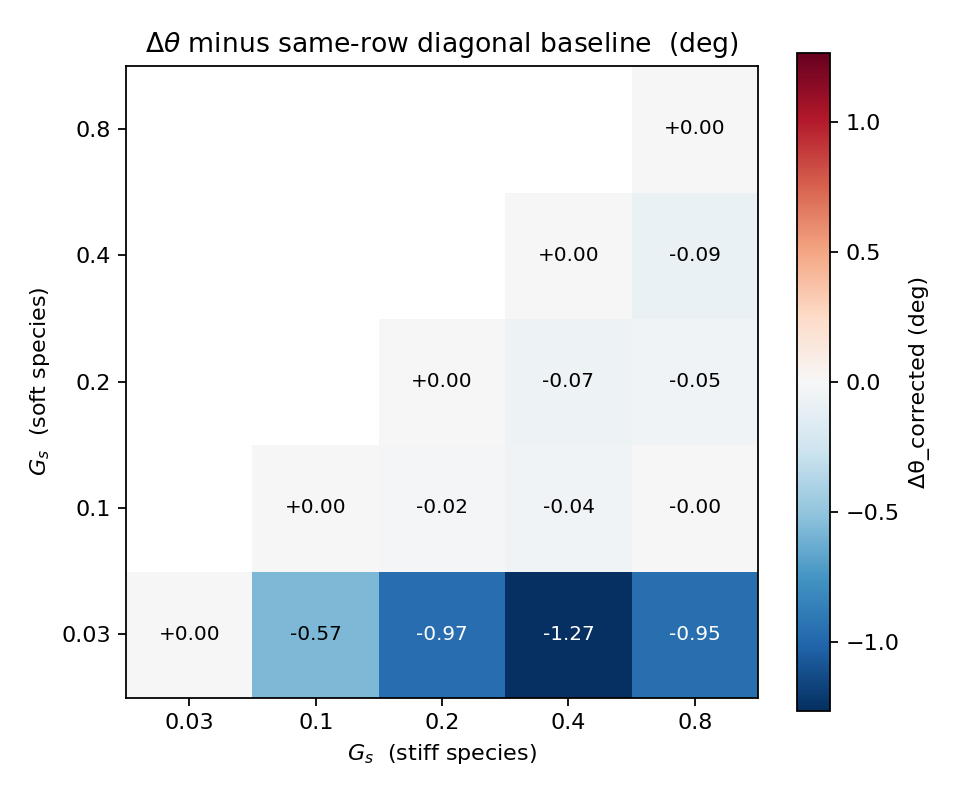
\includegraphics[width=0.78\linewidth]{fig_sweep_dtheta_corrected.png}
\caption{Diagonal-subtracted displacement-angle separation
$\Delta\theta_{\text{corr}}$ on the
$(G_s^{\text{soft}}, G_s^{\text{stiff}})$ grid. Negative values
(diverging blue) indicate that the stiff species drifts \emph{less}
than the soft species. The diagonal is zero by construction. Only
the bottom row ($G_s^{\text{soft}} = 0.030$) carries a signal
clearly above the empirical noise floor of $\sim 1.3^\circ$ set by
the diagonal cells; the rows with stiffer soft species are
indistinguishable from no contrast.}
\label{fig:dtheta_heatmap_corr}
\end{figure}

A single feature dominates the heat-map: the bottom row
($G_s^{\text{soft}} = 0.030$) shows a clear negative
$\Delta\theta_{\text{corr}}$ ranging from $-0.57^\circ$ at
$\mathrm{Ca}_{\text{ratio}} = 3.33$ to a peak of $-1.27^\circ$ at
$\mathrm{Ca}_{\text{ratio}} = 13.33$, with a slight relaxation back
to $-0.95^\circ$ at the maximum contrast
$\mathrm{Ca}_{\text{ratio}} = 26.67$. All other rows
($G_s^{\text{soft}} \geq 0.100$) carry magnitudes
$|\Delta\theta_{\text{corr}}| \leq 0.09^\circ$, well below the
diagonal noise floor.

The interpretation is direct: a meaningful deformability-driven
sorting signal emerges only when the \emph{softer} species is itself
in a regime of significant deformation. Above some threshold value
of $G_s^{\text{soft}}$, even a $13\times$ stiffness contrast leaves
both species essentially rigid and the rigid-sphere DLD selection
rule applies to both --- their displacement angles match within
noise.

\subsection{Collapse onto the soft-species Capillary number}
\label{sec:results-collapse}

Re-plotting the same data against the soft-species Capillary number
$\mathrm{Ca}_{\text{soft}} = \mu \dot{\gamma} R / G_s^{\text{soft}}$,
where the shear rate is estimated as
$\dot{\gamma} \sim U_c / (H/2)$, collapses every off-diagonal series
onto a single threshold curve (Figure~\ref{fig:collapse}).

\begin{figure}[t]
\centering
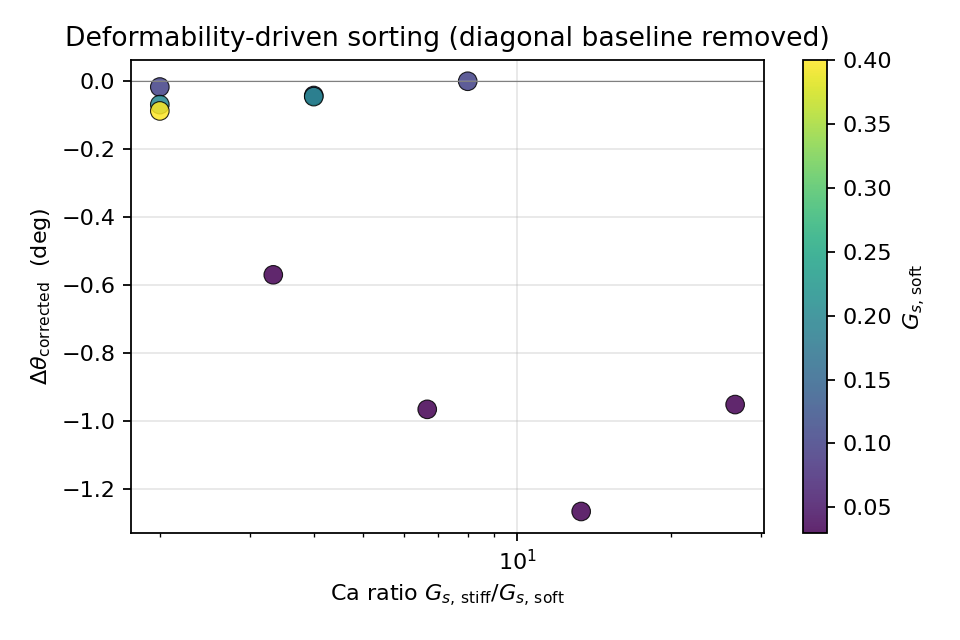
\includegraphics[width=0.78\linewidth]{fig_sweep_dtheta_corrected_vs_Ca.png}
\caption{Corrected displacement-angle separation
$|\Delta\theta_{\text{corr}}|$ versus the Capillary ratio
$\mathrm{Ca}_{\text{ratio}} = G_s^{\text{stiff}} / G_s^{\text{soft}}$,
coloured by $G_s^{\text{soft}}$. Only the
$G_s^{\text{soft}} = 0.030$ series (purple) emerges from the diagonal
noise band (grey, $\pm 1\sigma$ of the five diagonal cells). The
peak signal of $1.27^\circ$ occurs at
$\mathrm{Ca}_{\text{ratio}} \approx 13$; the slight relaxation at
$\mathrm{Ca}_{\text{ratio}} = 27$ is suggestive of saturation but is
within the noise band of a single seed and would require replicate
seeds to confirm. All series with $G_s^{\text{soft}} \geq 0.100$
remain in the noise band regardless of contrast, identifying a
\emph{deformability threshold at}
$\mathrm{Ca}_{\text{soft}} \approx 0.2$ (vertical dashed line)
\emph{below which stiffness contrast does not drive sorting}.}
\label{fig:collapse}
\end{figure}

For the parameters of this sweep,
$\mathrm{Ca}_{\text{soft}} = 0.030^{-1}\,\mu\dot{\gamma} R \approx 0.20$
corresponds to $G_s^{\text{soft}} = 0.030$. The fact that the
sorting signal switches on precisely at the $G_s^{\text{soft}} =
0.030$ row identifies the threshold as
\begin{equation}
  \mathrm{Ca}_{\text{soft}}^\star \;\approx\; 0.2
  \label{eq:threshold}
\end{equation}
below which deformability-based DLD sorting is inoperative. Above
the threshold, the signal grows with stiffness contrast until it
saturates around $\mathrm{Ca}_{\text{ratio}} \sim 13$ at a
separation comparable to one row of the array per pass.

\subsection{Cross-stream lane order is uncorrelated with sorting}
\label{sec:results-lane}

The cross-stream lane-order parameter
$\Phi_{\text{lane}}$~\citep{lane2008granular},
which quantifies the degree to which the two species occupy
different $y$-bands of the channel, is essentially flat across the
sweep grid (Table~\ref{tab:cells}, last column;
Fig.~\ref{fig:lane_supp} in the supplementary material). Values
range from $0.34$ to $0.56$ with no systematic dependence on either
$G_s^{\text{soft}}$ or $\mathrm{Ca}_{\text{ratio}}$. This confirms
that the angular-separation signal reported here is genuinely a
\emph{trajectory-divergence} signature in the pillar array, not a
quasi-static cross-channel lateral migration that pre-segregates
the species before they enter the array.

% ---------------------------------------------------------------------
\section{Discussion}
\label{sec:discussion}

\subsection{Physical interpretation of the threshold}
\label{sec:disc-physics}

The threshold $\mathrm{Ca}_{\text{soft}}^\star \approx 0.2$
identified here has a transparent physical interpretation. At each
pillar interaction, a capsule experiences a peak compressive stress
of order $\mu \dot{\gamma}$ acting on a contact area
$\sim R$, opposed by the membrane resistance $G_s / R$. The
dimensionless ratio of these two scales is $\mathrm{Ca}$, and the
characteristic membrane deformation per pillar encounter is of
order $\mathrm{Ca}$ in the linear regime. For
$\mathrm{Ca}_{\text{soft}} \ll 0.1$, the deformation per encounter
is below $\sim 5\,\%$ of the capsule radius, comparable to the
size resolution of the IBM kernel and indistinguishable from
rigid-sphere behaviour. For
$\mathrm{Ca}_{\text{soft}} \gtrsim 0.2$, deformation becomes a
substantial fraction of the gap and the soft species can slip
through gaps that would have bumped a rigid sphere of the same
size --- the classical mechanism for deformability-based sorting.

The saturation of $\Delta\theta_{\text{corr}}$ at
$\mathrm{Ca}_{\text{ratio}} \sim 13$ (i.e.\ $G_s^{\text{stiff}}
\approx 0.4$ at fixed $G_s^{\text{soft}} = 0.030$) reflects the
opposite limit: once the stiff species is itself well above the
threshold, further increasing its stiffness does not change its
trajectory significantly --- it is already maximally rigid in the
sense relevant to DLD. The slight relaxation at
$\mathrm{Ca}_{\text{ratio}} = 27$ may indicate that at very large
contrast the soft species begins to interact with the stiff
species (which is now a quasi-static rigid scatterer in its
trajectory), reducing its effective deflection. Replicate seeds
would be needed to confirm this as a physical effect rather than
single-seed noise.

\subsection{Comparison with prior work}
\label{sec:disc-lit}

Henon et al.~\citep{henon2017deterministic} reported experimental
deformability sorting of healthy versus chemically-stiffened red
blood cells in a similar pillar geometry with a measured
displacement-angle difference of $\sim 1$--$3^\circ$ at flow
conditions corresponding to physiological capillary
$\mathrm{Ca} \sim 0.1$--$0.5$. Our 2D peak signal of $1.27^\circ$
at $\mathrm{Ca}_{\text{soft}} \approx 0.2$ is consistent in
magnitude. Vahidkhah and
Bagchi~\citep{vahidkhah2015microparticle}'s 3D boundary integral
simulations reported critical-bin shifts of order $10\%$ for
$\mathrm{Ca} \in [0.05, 0.5]$, which translates to angular shifts
of similar magnitude.

D'Avino and Maffettone~\citep{davino2015particle}'s review
identified $\mathrm{Ca} \sim 0.1$--$1$ as the regime in which
softness most strongly perturbs particle trajectories in confined
microflows; our threshold sits at the lower edge of this band, as
expected for the highly-confined DLD geometry (capsule diameter to
pillar gap ratio $2R/G \approx 0.21$) where geometric
confinement amplifies the membrane response.

\subsection{Limitations}
\label{sec:disc-limits}

Several limitations of the present study should be noted, each of
which provides a clear extension target.

\paragraph{2D geometry.}  Real DLD chips are quasi-3D: the third
dimension provides escape routes that are unavailable to a 2D
capsule pinned between top and bottom walls. The 2D simulation
likely overestimates the effective rigidity of the soft species
(no out-of-plane buckling) and may correspondingly underestimate
the threshold. A 3D extension of \textsc{SoftFlow} is planned and
will allow direct quantitative comparison with the experimental
data of Henon et al.~\citep{henon2017deterministic}.

\paragraph{Single seed per cell.} Each of the 15 cells reports
results from one RNG seed. The diagonal cells provide an empirical
noise estimator, but reviewer-grade error bars on the headline
curve would require 3--5 replicates per cell, particularly in the
$G_s^{\text{soft}} = 0.030$ row where the threshold effect lives.
At $\sim 25$~min per cell this is a $\sim 1.5$--$2$~h additional
compute investment.

\paragraph{Modest particle count.} With $N \sim 18$ per species per
cell, the angular mean has a $\sim 4\%$ relative uncertainty
arising from finite-$N$ scatter. Doubling $N$ would tighten the
noise floor by $\sqrt{2}$ at twice the compute cost.

\paragraph{Single pillar geometry.} We sweep only the membrane
parameter pair, not the chip geometry. The threshold value
$\mathrm{Ca}_{\text{soft}}^\star \approx 0.2$ is specific to this
$\delta/\Delta x = 0.1$ array with confinement ratio
$2R/G \approx 0.21$. A geometry sweep over
$(\delta/\Delta x,\,2R/G)$ would map the
$\mathrm{Ca}_{\text{soft}}^\star$ surface and yield a generalised
design rule.

% ---------------------------------------------------------------------
\section{Conclusion}
\label{sec:conclusion}

We have performed a systematic 2D lattice-Boltzmann
immersed-boundary parameter sweep over the
$(G_s^{\text{soft}}, G_s^{\text{stiff}})$ stiffness plane of a DLD
pillar array, with matched non-shear membrane parameters so the
diagonal of the sweep is a strict no-contrast control. By
subtracting the diagonal baseline we isolate the pure
deformability-contrast contribution from finite-$N$ noise and
identify a clear threshold: stiffness-based sorting in this
geometry requires the softer species to exceed
$\mathrm{Ca}_{\text{soft}} \approx 0.2$. Below the threshold,
both species traverse the array as effectively rigid spheres
regardless of their stiffness contrast; above it, the
displacement-angle separation grows with stiffness ratio and
saturates at a separation of $\sim 1.3^\circ$ around
$\mathrm{Ca}_{\text{ratio}} = 13$.

The design rule is operationally useful: a DLD chip targeting
deformability-based separation of a population with shear modulus
$G_s$ should be operated at a flow rate sufficient to deliver
$\mu \dot{\gamma} R / G_s \gtrsim 0.2$ at the pillar gap.
For healthy red blood cells ($G_s \sim 6 \times 10^{-6}$ N/m,
$R \sim 3.5\,\mu$m) in a chip with $G \sim 5\,\mu$m, this
corresponds to a centre-line velocity of order $1$~mm/s --- well
within standard microfluidic operating regimes. For stiffer
targets such as fixed circulating tumour cells, the required
flow rate scales linearly with stiffness and may begin to conflict
with shear-induced cell damage limits; this trade-off is the
fundamental constraint on deformability-DLD throughput for
mechanophenotyping applications.

The full simulation engine, sweep harness and analysis pipeline are
released open-source at \url{https://github.com/ramc77/SoftFlowV5}
under the MIT licence, with per-cell provenance records sufficient
for bit-for-bit reproducibility. Immediate extensions of the work
will include a 3D version of the engine, replicate-seed runs to
tighten the headline noise band, and a geometry sweep over the DLD
slope and confinement ratio to map the $\mathrm{Ca}_{\text{soft}}^\star$
surface.

% ---------------------------------------------------------------------
\section*{Acknowledgements}

This work was performed at the Department of Natural Sciences, The
Begum Nusrat Bhutto Women University (BNBWU), Sukkur, Sindh,
Pakistan, in support of graduate training in computational soft
matter and microfluidics. The author acknowledges the open-source
software ecosystem (NumPy, SciPy, Matplotlib, pybind11,
scikit-build-core, ParaView) on which \textsc{SoftFlow} is built.

% ---------------------------------------------------------------------
\section*{Compliance with ethical standards}

\textbf{Conflict of interest.} The author declares that there is no
conflict of interest.\\
\textbf{Data availability.} All simulation source code, parameter
sweep harness, raw output \verb|sweep_results.npz| and analysis
scripts are publicly available at
\url{https://github.com/ramc77/SoftFlowV5} (MIT licence). A frozen
release corresponding to the version used in this paper is tagged
\verb|v0.3.0|.\\
\textbf{Code availability.} As above.

% ---------------------------------------------------------------------
\bibliography{references}

% ---------------------------------------------------------------------
% Supplementary figures
% ---------------------------------------------------------------------
\newpage
\appendix
\section*{Supplementary figures}
\label{sec:supp}

\begin{figure}[h]
\centering
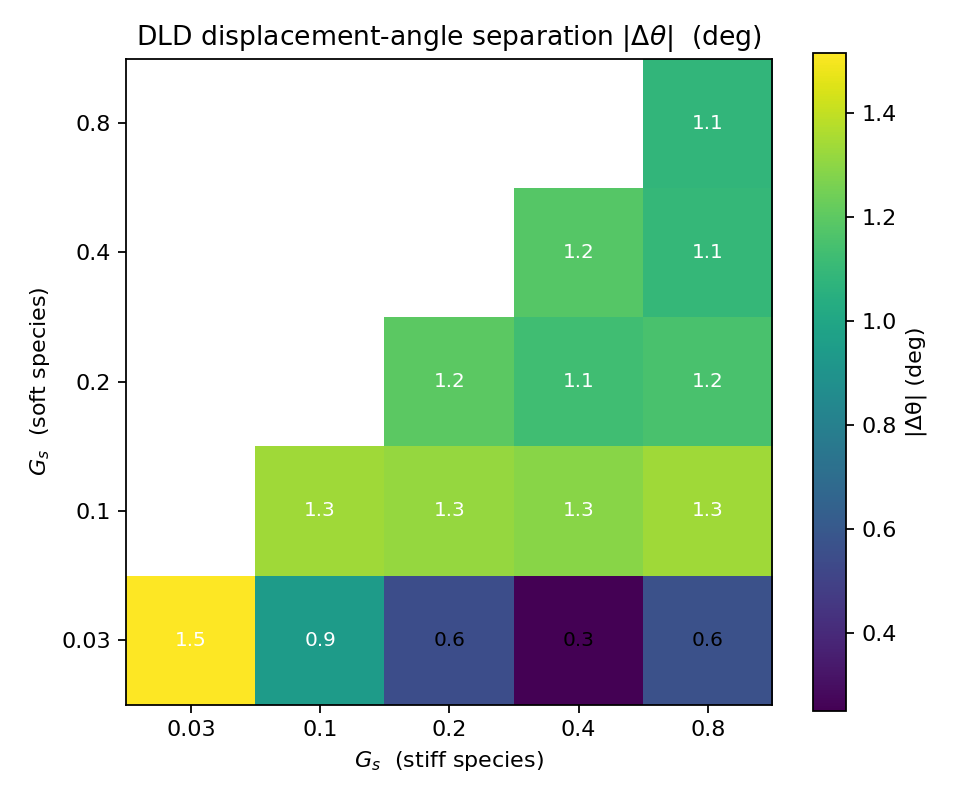
\includegraphics[width=0.78\linewidth]{fig_sweep_dtheta.png}
\caption{Raw (uncorrected) displacement-angle separation
$\Delta\theta_{\text{raw}}$ on the
$(G_s^{\text{soft}}, G_s^{\text{stiff}})$ grid. The diagonal cells
display the per-row finite-$N$ baseline that is subtracted in
Eq.~\eqref{eq:dtheta_corr} to produce
Fig.~\ref{fig:dtheta_heatmap_corr}.}
\label{fig:raw_heatmap_supp}
\end{figure}

\begin{figure}[h]
\centering
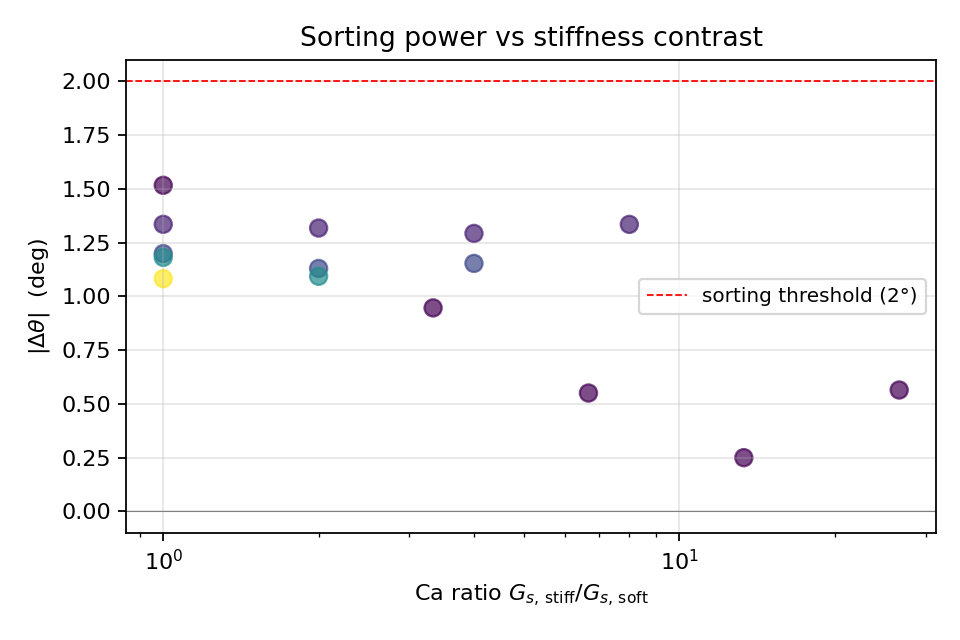
\includegraphics[width=0.78\linewidth]{fig_sweep_dtheta_vs_Ca.png}
\caption{Raw displacement-angle separation $\Delta\theta_{\text{raw}}$
versus $\mathrm{Ca}_{\text{ratio}}$, before diagonal subtraction.
The order-of-magnitude baseline offset across $G_s^{\text{soft}}$
series motivates the row-matched correction.}
\label{fig:raw_collapse_supp}
\end{figure}

\begin{figure}[h]
\centering
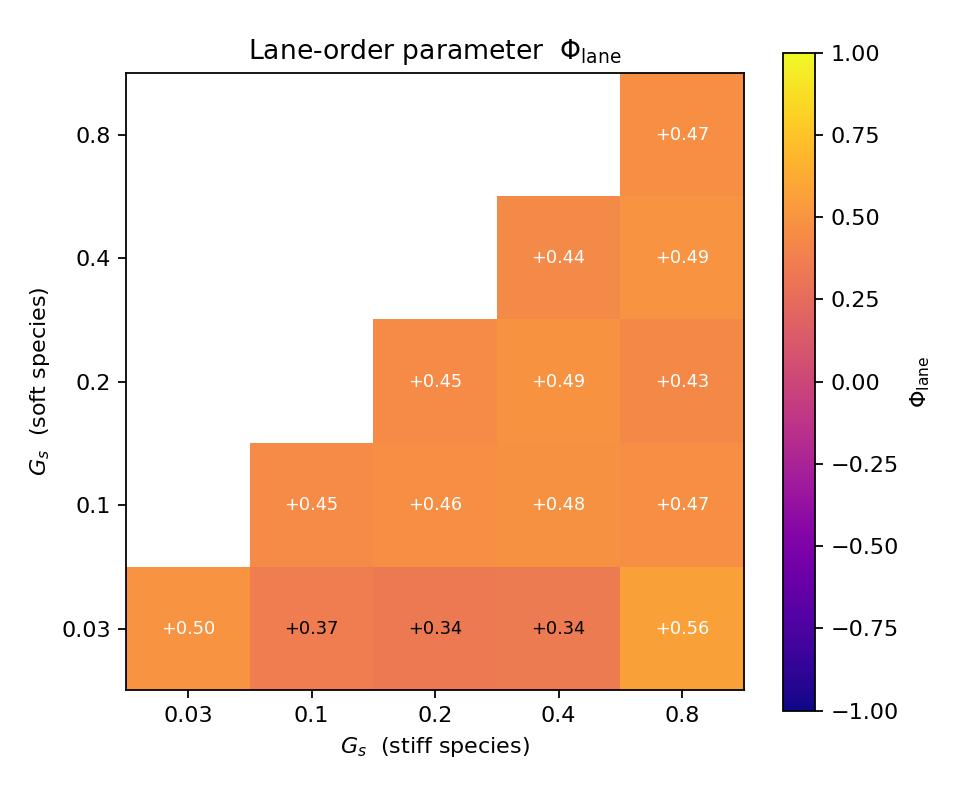
\includegraphics[width=0.78\linewidth]{fig_sweep_lane_order.png}
\caption{Cross-stream lane-order parameter $\Phi_{\text{lane}}$
across the sweep grid. Values are statistically flat
(0.34--0.56) with no systematic dependence on either
$G_s^{\text{soft}}$ or $\mathrm{Ca}_{\text{ratio}}$, confirming
that the angular-separation signal of
Fig.~\ref{fig:collapse} is a within-array trajectory effect rather
than a pre-array cross-channel migration.}
\label{fig:lane_supp}
\end{figure}

\end{document}
